\documentclass[border=2mm,tikz]{standalone}
\usetikzlibrary{positioning, fit, shapes.geometric}

\begin{document}
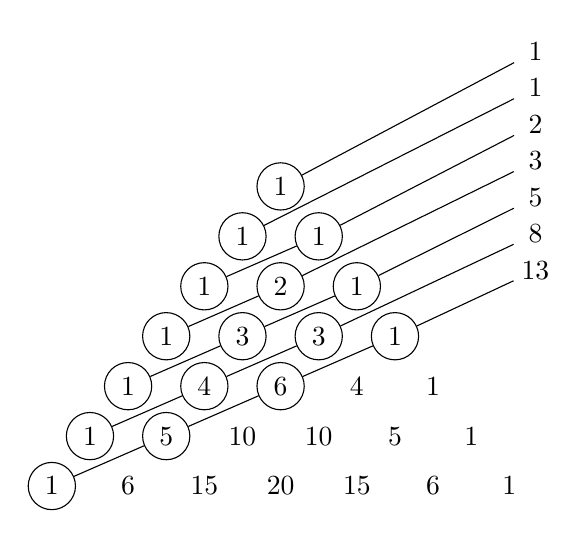
\begin{tikzpicture}[
circled/.style={draw=black},
every node/.style={circle, inner sep=0mm, minimum width=6mm, minimum height=6mm, align=center}]

\node[circled] (a1) {1};

\node[circled, below left=2mm and 0.5mm of a1] (b1) {1};
\node[circled, below right=2mm and 0.5mm of a1] (b2) {1};

\node[circled, below left=2mm and 0.5mm of b1] (c1) {1};
\node[circled, below left=2mm and 0.5mm of b2] (c2) {2};
\node[circled, below right=2mm and 0.5mm of b2] (c3) {1};

\node[circled, below left=2mm and 0.5mm of c1] (d1) {1};
\node[circled, below left=2mm and 0.5mm of c2] (d2) {3};
\node[circled, below left=2mm and 0.5mm of c3] (d3) {3};
\node[circled, below right=2mm and 0.5mm of c3] (d4) {1};

\node[circled, below left=2mm and 0.5mm of d1] (e1) {1};
\node[circled, below left=2mm and 0.5mm of d2] (e2) {4};
\node[circled, below left=2mm and 0.5mm of d3] (e3) {6};
\node[below left=2mm and 0.5mm of d4] (e4) {4};
\node[below right=2mm and 0.5mm of d4] (e5) {1};

\node[circled, below left=2mm and 0.5mm of e1] (f1) {1};
\node[circled, below left=2mm and 0.5mm of e2] (f2) {5};
\node[below left=2mm and 0.5mm of e3] (f3) {10};
\node[below left=2mm and 0.5mm of e4] (f4) {10};
\node[below left=2mm and 0.5mm of e5] (f5) {5};
\node[below right=2mm and 0.5mm of e5] (f6) {1};

\node[circled, below left=2mm and 0.5mm of f1] (g1) {1};
\node[below left=2mm and 0.5mm of f2] (g2) {6};
\node[below left=2mm and 0.5mm of f3] (g3) {15};
\node[below left=2mm and 0.5mm of f4] (g4) {20};
\node[below left=2mm and 0.5mm of f5] (g5) {15};
\node[below left=2mm and 0.5mm of f6] (g6) {6};
\node[below right=2mm and 0.5mm of f6] (g7) {1};

\node[above right=4mm and 13.5mm of d4] (sum7) {13};
\node[above=-1.5mm of sum7] (sum6) {8};
\node[above=-1.5mm of sum6] (sum5) {5};
\node[above=-1.5mm of sum5] (sum4) {3};
\node[above=-1.5mm of sum4] (sum3) {2};
\node[above=-1.5mm of sum3] (sum2) {1};
\node[above=-1.5mm of sum2] (sum1) {1};

\draw (a1) -- (sum1);
\draw (b1) -- (sum2);
\draw (c1) -- (b2) -- (sum3);
\draw (d1) -- (c2) -- (sum4);
\draw (e1) -- (d2) -- (c3) -- (sum5);
\draw (f1) -- (e2) -- (d3) -- (sum6);
\draw (g1) -- (f2) -- (e3) -- (d4) -- (sum7);

\end{tikzpicture}
\end{document}
